\chapter{Planejamento das Avaliações}

\begin{figure}[h!]
  \centering
    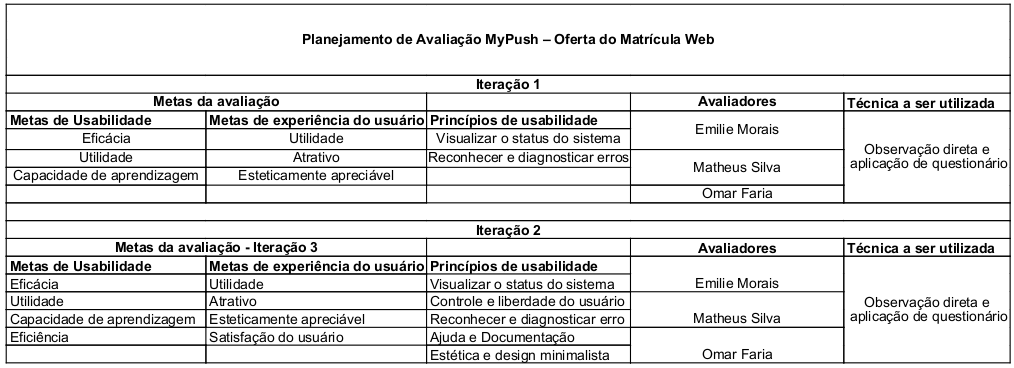
\includegraphics[keepaspectratio=true, scale=0.5]{figuras/planejamentoavaliacoes.png}
  \caption{Planejamento das avaliações}
\end{figure}

% \begin{figure}[h!]
%   \centering
%     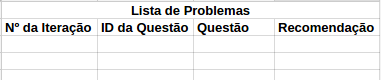
\includegraphics[keepaspectratio=true, scale=0.7]{figuras/listaproblemas.png}
%   \caption{Lista de problemas a ser preenchida nas avaliações}
% \end{figure}
% 
\begin{table*}[!h]
\caption{Lista de problemas a ser preenchida nas avaliações. Fonte: \cite{preece} adaptado}
\label{Rotulo}
  \begin{tabular}{p{0.18\linewidth}p{0.18\linewidth}p{0.30\linewidth}p{0.30\linewidth}}
  \hline
    Nº da Iteração & ID da Questão & Questão & Recomendação\\
 \hline
  \end{tabular}
\end{table*}
  
\pagebreak

\section{Iteração 1}

\begin{figure}[h!]
  \centering
    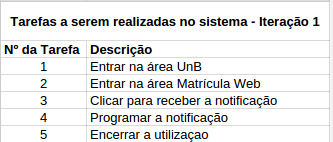
\includegraphics[keepaspectratio=true, scale=0.7]{figuras/tarefas1.png}
  \caption{Lista de Tarefas para os usuários na Iteração 1}
\end{figure}

\begin{table*}[!h]
\caption{Lista de problemas. Fonte: \cite{preece} adaptado}
\label{Rotulo}
  \begin{tabular}{p{0.18\linewidth}p{0.18\linewidth}p{0.30\linewidth}p{0.30\linewidth}}
  \hline
    Nº da Iteração & ID da Questão & Questão & Recomendação\\
 \hline
  \end{tabular}
\end{table*}